\subsection{Paid causal certificate controls}
\label{sec:certificateexperiment}
We repeat the 432 BT trajectories from Section~\ref{sec:multidata},
using the same 108 dataset/radius/vertex cases and four methods. All
original terminal values, certificates, update counts and oracle counts
match the earlier archive exactly. The five controls are scalar,
disjoint blocks of $K=8,32,128$, and known $\mu=0.01$, as defined in
Section~\ref{sec:tangentmonitors}. Block sizes are fixed before observing
the results. These give 2160 dependent causal stopping profiles, not
2160 independent optimization runs. No new data or starting points
are introduced.

The monitors see only paid source values and gradients; neither the
line search nor initialization changes. We record the first causal
prefix with certificate at most $10^{-5}$, or the original endpoint.
Twenty native online-stop checks on a synthetic interior instance verify
the prefix construction and actual oracle costs for every method/profile
pair. Each profile's isolated LMO cost includes its own block
queries and the direction queries, excluding the other monitors.
An affordable budget prefix must pay the entire scheduled verification
at its source. No incomplete block is queried, and references are not
monitor inputs. The original trajectory cap is retained.

All three block sizes fail to produce any earlier stop: each retains
129/432 successes. At the common original endpoint, $K=8$ improves
the certificate on 61 paths and $K=32$ on 22, but the improvements do
not cross the tolerance. Blocks increase total LMO cost on 432, 425,
and 380 paths, respectively. This negative control does not establish
failure of other weights, block sizes, or exact Fenchel dual evaluation.

The known-$\mu$ control gives 226/432 successes and 110 earlier
prefixes without additional LMOs. On interior Metro all four methods
certify 24/24 starts. FW's function-call medians become 746.5 and
724.5, versus censored scalar medians 2000 and 2002; AFW's become
481.5 and 458, versus 2000 and 2001. At the separate budget of
1000 function calls, FW has 18/24 and 15/24 successes, and both AFW
variants have 24/24. Interior Seoul remains difficult: AFW has 4/30
and 10/30 successes at the full cap, but none at 1000 function calls;
FW has none. Active-regime success counts are unchanged.

Thus a standard certificate using analytical model information resolves
much of the observed Metro stopping lag, while the tested first-order
block controls do not. The known-$\mu$ result is not evidence of
adaptation to unknown strong convexity or a new rate. The original
scalar-certificate bounds remain the main analytical claim.
Full-path audits check lower-bound validity, certificate monotonicity,
dominance over scalar, and the exact extra-LMO schedule before sampling.
Active-set scans remain additional work; no wall-clock comparison is made.

\begin{table}[htbp]
\centering\small
\caption{Interior causal stopping controls. Each cell is the certified count and median function calls up to its first stop or the original cap; censored cases are included. Seoul has 30 starts per method, Metro 24. $F/A$: FW/AFW; subscripts $1,U$: initial $M=1,U_0/D^2$. Blocks use one additional full LMO per completed block; the known-$\mu$ column receives extra problem information.}
\label{tab:certificates}
\begin{tabular}{llrrrrr}
\hline
Data & Method & Scalar & $K=8$ & $K=32$ & $K=128$ & Known $\mu$ \\
\hline
Seoul & $F_1$ & 0; 2001 & 0; 2001 & 0; 2001 & 0; 2001 & 0; 2001 \\
Seoul & $F_U$ & 0; 1996 & 0; 1996 & 0; 1996 & 0; 1996 & 0; 1996 \\
Seoul & $A_1$ & 0; 2001 & 0; 2001 & 0; 2001 & 0; 2001 & 4; 2001 \\
Seoul & $A_U$ & 0; 1995.5 & 0; 1995.5 & 0; 1995.5 & 0; 1995.5 & 10; 1995 \\
\hline
Metro & $F_1$ & 0; 2000 & 0; 2000 & 0; 2000 & 0; 2000 & 24; 746.5 \\
Metro & $F_U$ & 0; 2002 & 0; 2002 & 0; 2002 & 0; 2002 & 24; 724.5 \\
Metro & $A_1$ & 6; 2000 & 6; 2000 & 6; 2000 & 6; 2000 & 24; 481.5 \\
Metro & $A_U$ & 7; 2001 & 7; 2001 & 7; 2001 & 7; 2001 & 24; 458 \\
\hline
\end{tabular}
\end{table}

\begin{figure}[htbp]
\centering
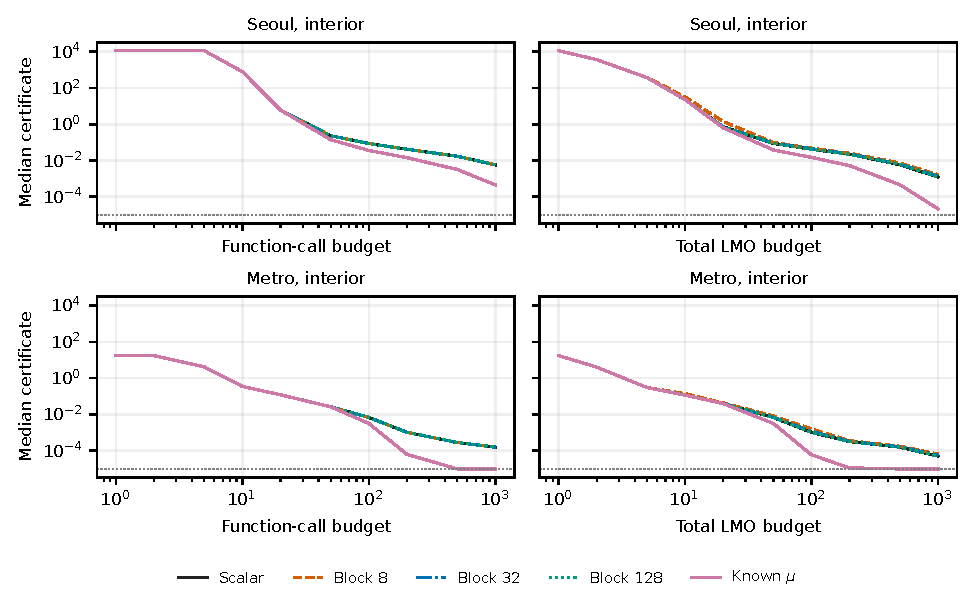
\includegraphics[width=\textwidth]{figures/causal_certificates.pdf}
\caption{Causal controls on interior AFW-BT paths with initial
$M=U_0/D^2$. Median certificates over all 30 Seoul or 24 Metro vertices
at separate function and total LMO budgets; total LMOs include the
profile's block queries. Completed prefixes are carried forward.
Known $\mu$ receives analytical ridge information; blocks do not.
All methods and both initializations appear in
Table~\ref{tab:certificates} and the archived report.}
\label{fig:causalcertificates}
\end{figure}
